%%%%%%%%%%%%%%%%%%%%%%%%%%%%%%%%%%%%%%%%%
% Short Sectioned Assignment
% LaTeX Template
% Version 1.0 (5/5/12)
%
% This template has been downloaded from:
% http://www.LaTeXTemplates.com
%
% Original author:
% Frits Wenneker (http://www.howtotex.com)
%
% License:
% CC BY-NC-SA 3.0 (http://creativecommons.org/licenses/by-nc-sa/3.0/)
%
%%%%%%%%%%%%%%%%%%%%%%%%%%%%%%%%%%%%%%%%%

%----------------------------------------------------------------------------------------
%	PACKAGES AND OTHER DOCUMENT CONFIGURATIONS
%----------------------------------------------------------------------------------------

\documentclass[paper=a4, fontsize=11pt]{scrartcl} % A4 paper and 11pt font size

\usepackage{graphicx}
\usepackage{float}
\usepackage{mathrsfs}
\usepackage[T1]{fontenc} % Use 8-bit encoding that has 256 glyphs
\usepackage{fourier} % Use the Adobe Utopia font for the document - comment this line to return to the LaTeX default
\usepackage[english]{babel} % English language/hyphenation
\usepackage{amsmath,amsfonts,amsthm} % Math packages

\usepackage{lipsum} % Used for inserting dummy 'Lorem ipsum' text into the template

\usepackage{sectsty} % Allows customizing section commands
\allsectionsfont{\centering \normalfont\scshape} % Make all sections centered, the default font and small caps

\usepackage{fancyhdr} % Custom headers and footers
\pagestyle{fancyplain} % Makes all pages in the document conform to the custom headers and footers
\fancyhead{} % No page header - if you want one, create it in the same way as the footers below
\fancyfoot[L]{} % Empty left footer
\fancyfoot[C]{} % Empty center footer
\fancyfoot[R]{\thepage} % Page numbering for right footer
\renewcommand{\headrulewidth}{0pt} % Remove header underlines
\renewcommand{\footrulewidth}{0pt} % Remove footer underlines
\setlength{\headheight}{13.6pt} % Customize the height of the header

\numberwithin{equation}{section} % Number equations within sections (i.e. 1.1, 1.2, 2.1, 2.2 instead of 1, 2, 3, 4)
\numberwithin{figure}{section} % Number figures within sections (i.e. 1.1, 1.2, 2.1, 2.2 instead of 1, 2, 3, 4)
\numberwithin{table}{section} % Number tables within sections (i.e. 1.1, 1.2, 2.1, 2.2 instead of 1, 2, 3, 4)

\setlength\parindent{0pt} % Removes all indentation from paragraphs - comment this line for an assignment with lots of text

%----------------------------------------------------------------------------------------
%	TITLE SECTION
%----------------------------------------------------------------------------------------

\newcommand{\horrule}[1]{\rule{\linewidth}{#1}} % Create horizontal rule command with 1 argument of height

\title{	
\normalfont \normalsize 
\textsc{RISE 2014} \\ [25pt] % Your university, school and/or department name(s)
\horrule{0.5pt} \\[0.4cm] % Thin top horizontal rule
\huge Derivations and Notes on Theory \\ % The assignment title
\horrule{2pt} \\[0.5cm] % Thick bottom horizontal rule
}

\author{Michael Matty} % Your name

\date{\normalsize\today} % Today's date or a custom date

\begin{document}

\maketitle % Print the title

%----------------------------------------------------------------------------------------
%	PART 1
%----------------------------------------------------------------------------------------

\section{Thermodynamic Quantities to First Order in Stillinger}

%------------------------------------------------

\subsection{Partition Function with Non-Interacting Monovacancies}
The general Stillinger expansion of the partition function takes the form
\begin{align}
  \label{eq:full-Q}
  Q = \frac{1}{\Lambda^{3N}} \sum\limits_l \prod\limits_i^N Z_i^l
      \prod\limits_{i<j}^N \frac{Z_{ij}^l}{Z_i^lZ_j^l} \cdots
\end{align}
Where the sum over l in (\ref{eq:full-Q}) denotes a sum over unique injective
mappings from natural numbers modulo the number of particles into the
natural numbers modulo the number of lattice sites (i.e. such that for
N many particles and M many lattice sites, two mappings are unique iff they do
not map onto the same cardinality N subset of $\mathbb{N}/M$).\\

Let us again assume that we have N particles and M lattice sites. To first
order in the Stillinger expansion, we include only the single particle
configuration integral product, and the sum over l just reduces to a
combinatorial factor counting the number of ways to place the N particles
among the M lattice sites.  Furthermore, let us assume that the interaction
potential is finitely ranged so that only particles within $n_m$ shells of a
given particle interact with it, and let $g_i$ be the number of particles
in shell i around a fixed site.  Then, for the $(M-N)$ vacancies,
$(M-N)g_i$ particles "feel" the vacancy at shell i.  Consequently,
$\sum\limits_i^{n_m} (M-N)g_i$ particles feel the effect of a vacancy,
while $N-\sum\limits_i^{n_m}(M-N)g_i$ do not.\\

For each of those particles that do not feel the effect of a vacancy, the 
configuration integral is identical, and is denoted $Z_s$.
For each of those particles that feel the effect of a vacancy at shell i,
the configuration integral is again identical and is denoted $Z_{sv,i}$.\\

Finally, this allows us to write the partition function to first order
as follows:
\begin{align}
  \label{eq:q1}
  \boxed{Q = \frac{1}{\Lambda^{3N}}\binom{M}{N} Z_s^{N-(M-N)\sum\limits_i^{n_m}g_i}
  \prod\limits_i^{n_m} Z_{sv,i}^{g_i(M-N)}}
\end{align}

\subsection{First Order Helmholtz Free Energy}
Now we examine the thermodynamic limit where $(N,M)\rightarrow\infty$ and
the particle number density $\rho\equiv N/V$ (where V is the volume) is held
constant. Letting the vacancy contration be given by $n_v \equiv 1-N/M$ and
using Stirling's approximation ($\ln(N!) \approx N\ln(N)-N$),
we have that:
\begin{align}
  \frac{\beta F}{N} &= \frac{-\ln(Q)}{N}\\ 
    &= \frac{-1}{N}\left( -N\ln(\Lambda^3)+\ln\left(\frac{M!}{N!(M-N)!}\right)
                      +\ln(Z_s)\left(N-(M-N)\sum\limits_i^{n_m}g_i\right)
                      +\sum\limits_i^{n_m}g_i(M-N)\ln(Z_{sv,i})\right) \\    
    &= \frac{-1}{N}\left(N\ln\left(\frac{Z_s}{\Lambda^3}\right) + 
       (M-N)\sum\limits_i^{n_m}g_i\ln\left(\frac{Z_{sv,i}}{Z_s}\right) + 
     M\ln(M)-N\ln(N)-(M-N)\ln(M-N)\right)\\
    &= -\ln\left(\frac{Z_s}{\Lambda^3}\right) - 
       \left(\frac{n_v}{1-n_v}\right)\sum\limits_i^{n_m}g_i
                                     \ln\left(\frac{Z_{sv,i}}{Z_s}\right)+
                                     (M/N-1)\ln(n_v)+\ln(1-n_v)\\
  \label{eq:1pfe}
  &= \boxed{-\ln\left(\frac{Z_s}{\Lambda^3}\right) - 
       \left(\frac{n_v}{1-n_v}\right)\sum\limits_i^{n_m}g_i
                                     \ln\left(\frac{Z_{sv,i}}{Z_s}\right)+
        \left(\frac{n_v}{1-n_v}\right)\ln(n_v)+\ln(1-n_v)}
\end{align}


\subsection{First Order Equilibrium Vacancy Concentration}
To obtain an expression for the equilibrium vacancy concentration, we must
minimize the free energy per particle wrt $n_v$.  Here, we assume that
$n_v \ll 1$, and thus we only keep terms whicha are independent of or
logarithmic in $n_v$.  Thus, proceeding from equation \ref{eq:1pfe}, we have:\\
\begin{align}
  \beta\frac{\partial(F/N)}{\partial n_v} &= 
  \frac{-\Lambda^3}{Z_s}\frac{1}{\Lambda^3}\frac{\partial Z_s}{\partial n_v}-
  \frac{1}{(1-n_v)^2}\sum\limits_i^{n_m}g_i \ln\left(\frac{Z_{sv,i}}{Z_s}\right)+
  \frac{1}{(1-n_v)^2}\ln(n_v) + \cdots\\
  &\approx \frac{-1}{Z_s}\frac{\partial Z_s}{\partial \rho}
  \frac{\partial\rho}{\partial n_v} - 
  \sum\limits_i^{n_m} g_i \ln\left(\frac{Z_{sv,i}}{Z_s}\right) + \ln(n_v)\\
  &= \frac{-1}{Z_s}\frac{\partial Z_s}{\partial \rho}\frac{\rho}{(1-n_v)^2}-
  \sum\limits_i^{n_m} g_i \ln\left(\frac{Z_{sv,i}}{Z_s}\right) + \ln(n_v)\\
  &\approx -\rho\frac{Z_s'}{Z_s} - 
  \sum\limits_i^{n_m} g_i \ln\left(\frac{Z_{sv,i}}{Z_s}\right) + \ln(n_v) = 0\\
  \label{eq:1pnveq}
  &\Rightarrow \boxed{n_{v,eq} = \exp\left(\rho\frac{Z_s'}{Z_s}\right)
  \prod\limits_i^{n_m}\left(\frac{Z_{sv,i}}{Z_s}\right)^{g_i}}
\end{align}

\subsection{First Order Gibb's Free Energy of Monovacancy Formation}
For small $n_{v,eq}$, $\beta F \approx -N\ln\left(\frac{Z_s}{\Lambda^3}\right)
\Rightarrow (F/N)' \approx -\beta^{-1} (Z_s'/Z_s)$.  Since the pressure, $p$,
is given by $p = (F/N)' \rho^2$, and using the relation
$n_{v,eq} = \exp(-\beta\Delta G_v)$ (where $\Delta G_v$ is the energy of 
monovacancy formation), it follows directly that:\\
\begin{align}
  \label{eq:1pdg}
  \boxed{\Delta G_v = \frac{p}{\rho}-
  \beta^{-1}\sum\limits_i^{n_m}g_i\ln\left(\frac{Z_{sv,i}}{Z_s}\right)}
\end{align}

%------------------------------------------------

\section{Thermodynamic Quanitites to Second Order In Stillinger}
\subsection{Second Order, No Vacancy Helmholtz Free Energy}
In the case of no vacancies, the sum in the partition function has only one
term as in this case any mapping is surjective.  Therefore, in the case of no
vacancies, the partition function to second order is
\begin{align}
  Q = \frac{1}{\Lambda^{3N}}\prod\limits_i^N Z_i\prod\limits_{i<j}^N
  \frac{Z_{ij}}{Z_iZ_j}
\end{align}

For no vacancies, each single particle integral is equivalent, i.e. in equation
\ref{eq:full-Q} we have $\forall i,j, Z_i = Z_j \equiv Z_s$.  Furthermore, each
two particle integral $Z_{ij}$ where the particle with label j is in the
kth shell of that with label i can be written identically as
$Z_{nk}$.  If $k > n_m$ (where $n_m$ is defined as in \ref{eq:q1}), then
$Z_{ij} = Z_i Z_j = Z_s^2$. Proceeding with this notation, we have:
\begin{align}
  \beta F &= -\ln(Q)\\
          &= -\ln\left(\frac{1}{\Lambda^{3N}}\right)
            -\sum\limits_{i=1}^N\ln(Z_s)-
             \sum\limits_{i=1}^N\sum\limits_{j=1}^{i-1}(\ln(Z_{ij})-\ln(Z_s^2))\\
          &= -N\ln\left(\frac{Z_s}{\Lambda^3}\right)+
             2\frac{1}{2}N(N-1)\ln(Z_s)-
             \sum\limits_{i=1}^N\sum\limits_{j=1}^{i-1}\ln(Z_{ij})
\end{align}

Now for each particle i (of which there are N many), there are $g_k$ particles
j in its kth shell.  Note that i is then also in the kth shell of each j. This
gives that there are $\frac{N}{2}g_k$ unique $i,j$ pairs representing
particles in each other's kth shell.  this allows us to proceed as follows:

\begin{align}
  &= -N\ln\left(\frac{Z_s}{\Lambda^3}\right)
     +(N^2-N)\ln(Z_s)-\left(\frac{N}{2}\sum\limits_{k=1}^{n_m}g_k\ln(Z_{nk})+
     \left(\frac{1}{2}(N^2-N)-\frac{N}{2}\sum\limits_{k=1}^{n_m}g_k\right)\ln(Z_s^2)\right)\\
  &= -N\ln\left(\frac{Z_s}{\Lambda^3}\right)
      -\frac{N}{2}\sum\limits_{k=1}^{n_m}g_k\ln(Z_{nk}) +
      N\sum\limits_{k=1}^{n_m}g_k \ln(Z_s)\\
  \label{eq:2pfe}
  &\Rightarrow \boxed{\frac{\beta F}{N} = -\ln\left(\frac{Z_s}{\Lambda^3}\right)-
   \frac{1}{2}\sum\limits_{k=1}^{n_m} g_k \ln\left(\frac{Z_{nk}}{Z_s^2}\right)}
\end{align}

It is interesting to note that this takes the form of the one particle
Helmholtz free energy per particle (c.f. equation \ref{eq:1pfe}) in the case
that $n_v \rightarrow 0$, with additional corrections concerning
the correlated movement of two particles at each relevant layer separation.

\subsection{Second Order Helmholtz Free Energy For Hard Spheres}
In the case of hard spheres, only nearest neighbor particles can interact
(i.e. $n_m = 1$).
Consequently, there are only two types of single
particle integrals.  Namely, for a particle in shell i of a vacancy, the
single particle integral is $Z_s$ if $i > 1$ or $Z_{sv,1} \equiv Z_{sv}$
otherwise.\\

There are, however, several types of two-particle integrals.
First note that if two particles labelled i and j are separated by more than one shell,
it is the case that $Z_{ij}^l = Z_{i}^lZ_{j}^l$, and consequently,
$\frac{Z_{ij}^l}{Z_i^lZ_j^l} = 1$, so such cases are irrelevant.
If the two moving particles are nearest-neighbors, then either neither of
those two are the nearest neighbor of a vacancy (in which case we denote
the two particle integral $Z_{ss}$), both of them are the nearest neighbor of
a vacancy (in which case we denote the two particle integral $Z_\alpha$), or
only one of them is the nearest neighbor of a vacancy.  In this final case,
there are three subcases to consider.  In particular, the moving particle that
is not a nearest neighbor of the vacancy can be in the second, third, or 
fourth shell of the vacancy, where these two particle integrals will be
denoted $Z_\delta$,$Z_\gamma$, and $Z_\beta$ respectively.  These different 
cases are illustrated in figure 2.1 below.

\begin{figure}[H]
  \centering
  \label{fig:int-labels}
  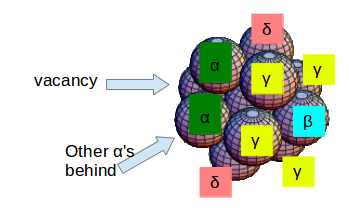
\includegraphics[scale=0.75]{integral_labels.png}
  \caption{This figure illustrates the different cases of two-particle
           integrals for hard spheres with a vacancy as the nearest neighbor
           to at least one of the moving particles. The vacancy is labelled
           on the right, and the first moving particle is in the center of
           the cluster, unlabelled.  The integral types for the case of each
           non vacant nearest neighbor site of the first moving particle
           being the second moving particle are denoted}
\end{figure}

As can be seen in figure 2.1, for each vacancy there are four $Z_\alpha$ 
type integrals, one $Z_\beta$, four $Z_\gamma$ and two $Z_\delta$ type
integrals per nearest neighbor.  Therefore, since each vacancy has twelve
nearest neighbors, there are twelve time each of these counts for each type
for each vacancy, excepting the $Z_\alpha$ type integrals which are counted
twice this way since each moving particle involved is a nearest neighbor of
the vacancy, yielding a factor of a half in the total count of $Z_\alpha$
integrals.  It remains for us to count the $Z_{ss}$ type integrals.  To do so,
first note that for N particles and no vacancies, there are $6N$ unique nearest neighbor 
pairs of particles as each particle 
has twelve nearest neighbors, but we must divide by two as pair $i,j$ is not
distinct from pair $j,i$.  Now if we have M sites, for each of (M-N) vacancies, twelve nearest
neighbor pairs are removed.  The number of remaining nearest neighbor pairs neither
of which are nearest neighbors of a vacancy can then be found by subtracting
the integral counts above from the total number of nearest neighbor pairs,
yielding $(6N-12(M-N))-108(M-N)$ many $Z_{ss}$ integrals.\\

Let us now define $\mathscr{Z}_\alpha \equiv \frac{Z_\alpha}{Z_{sv}Z_{sv}}$,
$\mathscr{Z}_\beta \equiv \frac{Z_\beta}{Z_{sv}Z_s}$,
$\mathscr{Z}_\gamma \equiv \frac{Z_\gamma}{Z_{sv}Z_s}$, and
$\mathscr{Z}_\delta \equiv \frac{Z_\delta}{Z_{sv}Z_s}$.
Assuming once more that we have M sites and N particles, we 
can then write the second order partition function as follows
(assuming again of course that the vacancies are placed far enough apart
 as to be non-interacting):

\begin{align}
  \label{eq:2phsq}
  Q_2 = Q_1 \mathscr{Z}_\alpha^{24(M-N)}\mathscr{Z}_\beta^{12(M-N)}
            \mathscr{Z}_\gamma^{48(M-N)}\mathscr{Z}_\delta^{24(M-N)}
            \left(\frac{Z_{ss}}{Z_sZ_s}\right)^{(6N-12(M-N))-108(M-N)}
\end{align}

Where $Q_1$ is given by equation \ref{eq:q1}. Note that as we know the count
of each type of integral independent of configuration, the sum over l in 
equation \ref{eq:full-Q} has once again reduced to a simple binomial coefficient.\\

The Helmholtz free energy can then easily be obtained from equation
\ref{eq:2phsq} as follows:

\begin{align}
  \frac{\beta F_2}{N} &= -\ln(Q_2)/N\\
                      &= -\frac{\ln(Q_1)}{N} - \frac{1}{N}\left((M-N)\left(
                         24\ln(\mathscr{Z}_\alpha) + 12\ln(\mathscr{Z}_\beta) + 
                         48\ln(\mathscr{Z}_\gamma) + 24\ln(\mathscr{Z}_\delta)- 
                       120\ln\left(\frac{Z_{ss}}{Z_sZ_s}\right)\right)+
                         6N\ln\left(\frac{Z_{ss}}{Z_sZ_s}\right)\right)\\
                      &= -\frac{\ln(Q_1)}{N} - \left(\frac{n_v}{1-n_v}\right)\left(
                         24\ln(\mathscr{Z}_\alpha) +
                         12\ln(\mathscr{Z}_\beta) +
                         48\ln(\mathscr{Z}_\gamma) + 
                         24\ln(\mathscr{Z}_\delta) -
                         120\ln\left(\frac{Z_{ss}}{Z_sZ_s}\right)\right)-
                         6\ln\left(\frac{Z_{ss}}{Z_sZ_s}\right)
\end{align}

\subsection{Second Order Formation Energy for Hard Spheres}
We will again determine an expression for the Gibb's free energy of monovacancy
formation by minimizing the free energy with respect to the monovacancy
concentration.  We use the same assumption that $n_v \ll 1$, and thus ignore
terms that are not logarithmic in or independent of $n_v$.  
For notational brevity, let us define the set $I = \{\alpha,\beta,\gamma,\delta\}$ and allow
$n_i$ for $i \in I$ to denote the multiplicity of integrals of type $Z_i$.
We then proceed from the results of the section 2.2 as follows:

\newcommand{\szi}{\sum\limits_{i \in I} n_i \ln(\mathscr{Z}_i)}
\newcommand{\zss}{\ln\left(\frac{Z_{ss}}{Z_sZ_s}\right)}
\newcommand{\pd}[2]{\frac{\partial #1}{\partial #2}}
\begin{align}
  \begin{split}
  \frac{\beta\partial(F_2/N)}{\partial n_v} &=
  \beta\pd{(F_1/N)}{n_v} - 
  \frac{1}{(1-n_v)^2}\szi + \\ &\frac{120}{(1-n_v)^2}\zss - 
  6\frac{Z_sZ_s}{Z_{ss}}\left(\frac{\partial Z_{ss}}{\partial n_v}\frac{1}{Z_s^2} - 
                              2\frac{Z_{ss}}{Z_s^3}\frac{\partial Z_s}{\partial n_v}\right) +
  \cdots
  \end{split}\\
  &\approx -\frac{1}{Z_s}\pd{Z_s}{n_v}-12\ln\left(\frac{Z_{sv}}{Z_s}\right)+\ln(n_v)-
  \szi+120\zss-6\left(\frac{1}{Z_{ss}}\pd{Z_{ss}}{n_v}-\frac{2}{Z_s}\pd{Z_s}{n_v}\right)
\end{align}

Recalling from section 1.3 that $\pd{Z_s}{n_v} \approx \rho Z_s'$, and noting
that similarly $\pd{Z_{ss}}{n_v} \approx \rho Z_{ss}'$, we have that:

\begin{align}
  \beta\pd{(F_2/N)}{n_v} &\approx 11\rho\frac{Z_s'}{Z_s}-6\rho\frac{Z_{ss}'}{Z_{ss}}-
  12\ln\left(\frac{Z_{sv}}{Z_s}\right)-\szi+120\zss+\ln(n_v)
\end{align}

Setting this equalt zero and solving for $n_v$ yields our new expression for
$n_{v,eq}$:

\begin{align}
  \boxed{
  \label{eq:2phsnveq}
  n_{v,eq} = \exp\left(-11\rho\frac{Z_s'}{Z_s}\right)
             \exp\left(6\rho\frac{Z_{ss}'}{Z_{ss}}\right)
             \left(\frac{Z_{sv}}{Z_s}\right)^{12}
             \left(\frac{Z_{ss}}{Z_sZ_s}\right)^{120}
             \prod\limits_{i\in I}\mathscr{Z}_i^{n_i}
  }
\end{align}

For small $n_{v,eq}$, $\beta F \approx -N\ln(Z_s)-6N\zss \Rightarrow
(F/N)' \approx \beta^{-1}\left(11\frac{Z_s'}{Z_s}-6\frac{Z_{ss}'}{Z_{ss}}\right)$.
Once again using the relations $n_{v,eq} = \exp(-\beta\Delta G_v)$ and
$p = (F/N)'\rho^2$, we quickly arrive at our final result:

\begin{align}
  \label{eq:2phsdg}
  \boxed{
  \Delta G_v = \frac{p}{\rho} - \beta^{-1}\left(
               12\ln\left(\frac{Z_{sv}}{Z_s}\right)-
           120\zss+\szi\right)}
\end{align}

Like the one particle result, this expression can be decomposed into an equation
of state piece (the first term), and a configuration integral piece (the second term).
Note also that the second term takes the form of the one particle result for hard spheres
(the leftmost term inside the parentheses) and corrections from two particle integrals
(the rightmost two terms).

\section{Vacancy Interaction}
\subsection{Helmholtz Free Energy Shift}
In this section, we are interested in deriving the difference in free energy
between two vacancies at some finite separation and two non-interacting vacancies.
Let every particle within $n_m$ shells of a vacancy "feel" the effect of the
vacancy.  Let $\sum\limits_{i=1}^{n_m} g_i = \xi$, where $g_i$ is the number
of particles in shell i. Let the number of particles that are simultaneously
within $n_m$ shells of both vacancies, where the vacancies are separated by
k shells, be denoted $\xi_k'$.  We will denote the different kinds of integrals
for particles that can feel both vacancies as $Z_{sv,ij}$ where i is the
shell of the first vacancy that the particle is in, and j that of the second.
In the case of interacting vacancies separated by k shells, there will be 
$\xi_k'$ many more integrals of $Z_s$ type than in the case of non-interacting
vacancies, and for each $Z_{sv,ij}$, of which there are also $\xi_k'$ many,
there will be one fewer $Z_{sv,i}$ and one fewer $Z_{sv,j}$.  The first equation below is then the free energy for two non-interacting vacancies.  The second equation is that for two interacting vacancies.  The final equation is the difference between the free
energy in these two scenarios, where the outer sum is over the the possible second vacancies at a given separation (all of these terms should be the same) and the inner sum is over the particles in the overlap, of which there should be $\xi'_k$ for vacancies at separation k.

\begin{align}
  \beta F = -\sum\limits_{i=1}^{n_m} g_i \ln(Z_{sv,i}) - 
             \sum\limits_{j=1}^{n_m} g_j \ln(Z_{sv,j}) + \cdots\\
  \beta F = -\sum\limits_{i,j}\ln(Z_{sv,ij})-\xi'\ln(Z_s) + \cdots\\
  \Delta F = \sum\sum \ln\left(\frac{Z_{sv,ij}Z_s}{Z_{sv,i}Z_{sv,j}}\right)
\end{align}

%\subsection{Free Energy Minimization in the Presence of Monovacancies and
%            Divacancies (Unifinished)}

\end{document}
